\chapter{Über Claus Bernet}

\begin{floatingfigure}[l]{0.33\textwidth}
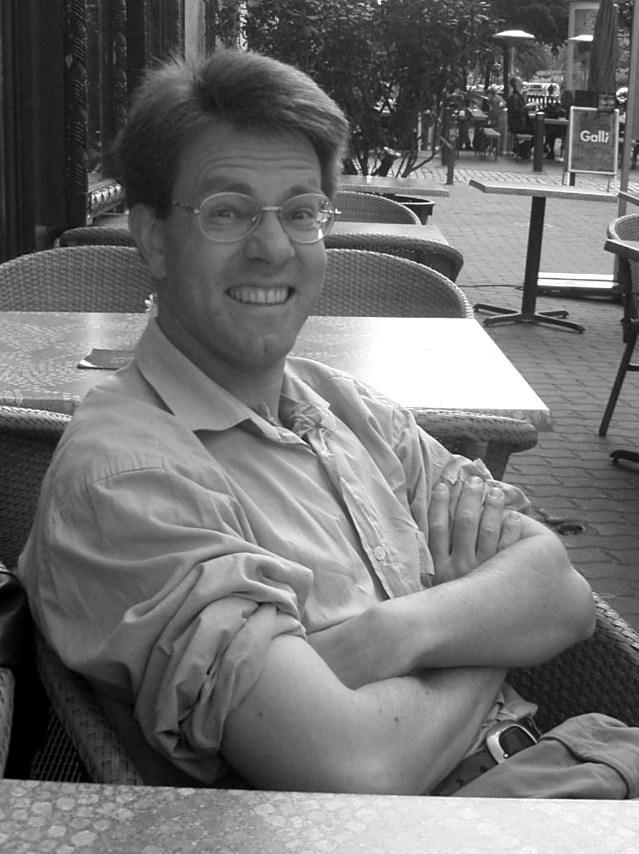
\includegraphics[width=0.33\textwidth]{claus_bernet_bw}
\end{floatingfigure}

Claus Bernet studierte Geschichtswissenschaften, Kunstgeschichte und
Stadtplanung in Berlin, Wien und Birmingham (UK). Die Dissertation erfolgte 2005
an der Martin-Luther-Universität Halle im Bereich Frühe Neuzeit.

\medskip

Parallel studierte er Erziehungswissenschaften an der Freien Universität Berlin.
2007 promovierte er mit einer Arbeit zur Erziehungsgedanken in nichtstaatlichen
Einrichtungen.

\medskip

Beschäftigung zu Themen der Gewaltprävention (PAG) und zur neosokratischen
Gesprächsführung; 2002/03 Mitarbeit beim Zentrum für Demokratische Kultur in
Berlin. 2008/09 koordinierte Bernet des Interview-Projektes "`Erweckte
Geschichte"'.

\medskip

Derzeit Arbeit er an einer Studie zu deutsch-italienischen Intellektuellen um
1900 mit einem Stipendiat des Literaturarchivs Marbach 2008. Desweiteren ist er
seid Jahren tätig als Mitarbeiter für die Lebenshilfe e.V. in Berlin.

\medskip

Die Forschungsgebiete von Claus Bernet sind historische Friedenskirchen,
Pietismus, Stadtgeschichte und Genossenschaftswesen.

\medskip

Folgende Veröffentlichungen zur Quäkerforschung sind bisher von Bernet
erschienen:

\begin{itemize}
 \item Rufus Jones (1863-1948). Life and Bibliography of an American Scholar,
Writer, and Social Activist. With a Foreword by Douglas Gwyn, New York 2009.
 \item Quäker aus Politik, Kunst und Wissenschaft in Deutschland. 20.
Jahrhundert. Ein biographisches Lexikon, Nordhausen 2007. 2. Auflage Nordhausen
2008. 3. Auflage in Planung.
 \item Between Quietism and Radical Pietism: The German Quaker Settlement
Friedensthal. 1792-1814, Birmingham 2004 (Woodbrooke Journal Series, 14).
\end{itemize}

\medskip


Claus Bernet ist Herausgeber der Reihe \textit{"`Deutsche Quäkerschriften"'}. Er
hält Vorträge in Deutschland, UK und USA zu Themen der Geschichte und Theologie
der Quäker. Ist Mitglied im Board of Trustees der englischen
Weiterbildungseinrichtung Woodbrooke in Birmingham seit 2004. Zahlreiche
Beiträge von ihm sind in der Zeitschrift "`Quäker"' -- dem Organ der Deutschen
Jahresversammlung e.V. -- erschienen.

\medskip

\begin{center}
\parbox{7,5cm}{
Tauroggener Str.2
\\10589 Berlin
\\bernet2@web.de
}
\end{center}